\chapter{Exemplo prático}

\section{Primeira aplicação - Contatos}

Baseado em \ref{sssec:testando} Testando o ADT, crie um novo aplicativo
chamado \textbf{Contatos}. Use \texttt{guia.android.exemplo} como o nome
da companhia. Siga os passos descritos nas figuras
\ref{fig:new-project-1}, \ref{fig:new-project-2},
\ref{fig:new-project-3} e \ref{fig:new-project-4} para criar uma
\texttt{Activity} inicial chamada \texttt{MainActivity} e um
\emph{layout} inicial chamado \texttt{main}. Depois clique em
\texttt{Finish}.

\begin{figure}[h]
    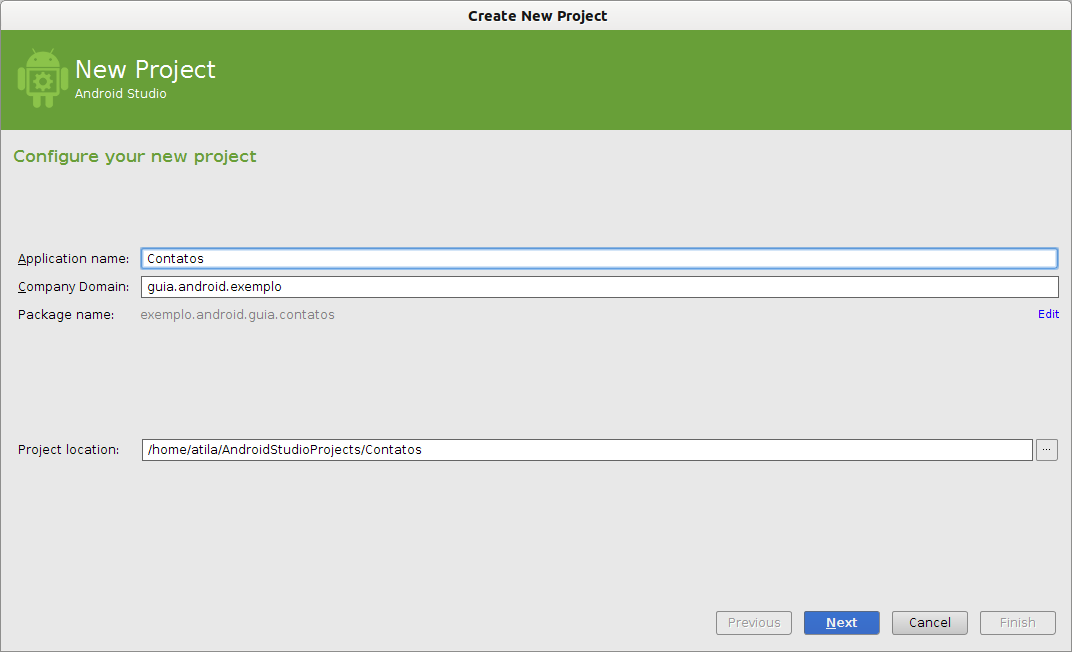
\includegraphics[scale=0.35]{img/exemplo-pratico/android-new-project-1.png}
    \caption{Novo projeto, tela 1}
    \label{fig:new-project-1}
\end{figure}

\begin{figure}[p]
    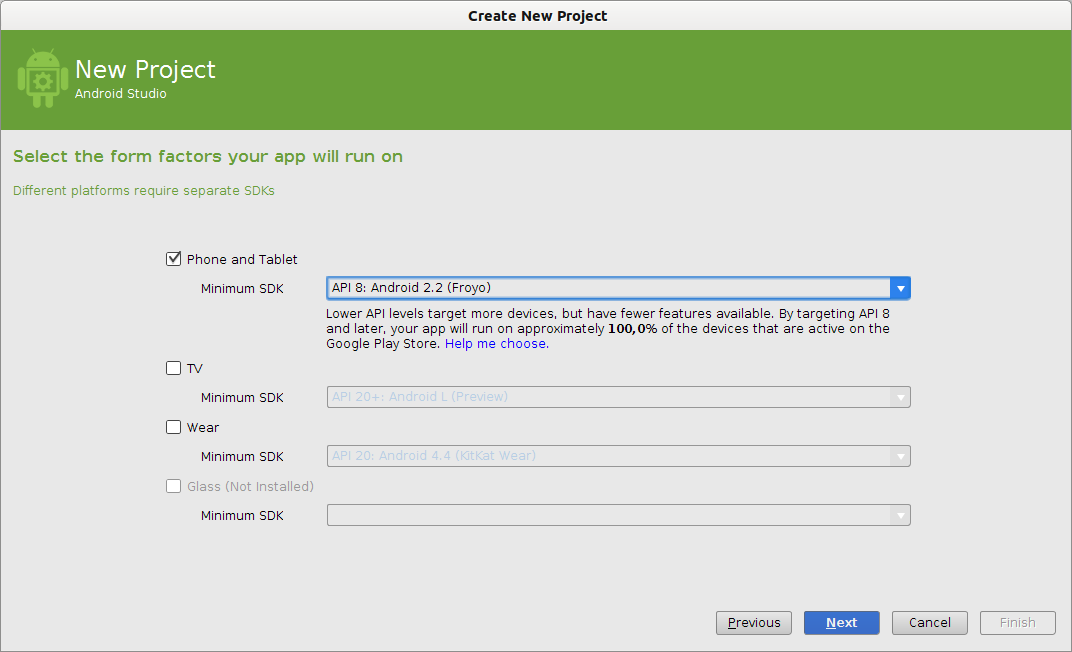
\includegraphics[scale=0.35]{img/exemplo-pratico/android-new-project-2.png}
    \caption{Novo projeto, tela 2}
    \label{fig:new-project-2}
\end{figure}

\begin{figure}[p]
    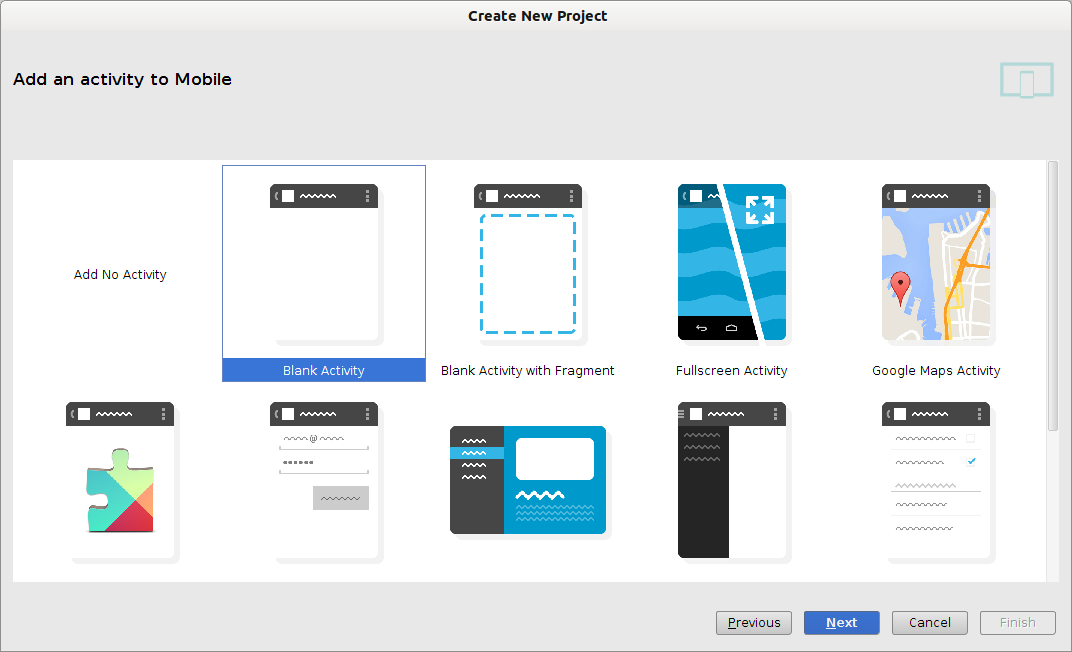
\includegraphics[scale=0.35]{img/exemplo-pratico/android-new-project-3.png}
    \caption{Novo projeto, tela 3}
    \label{fig:new-project-3}
\end{figure}

\begin{figure}[h]
    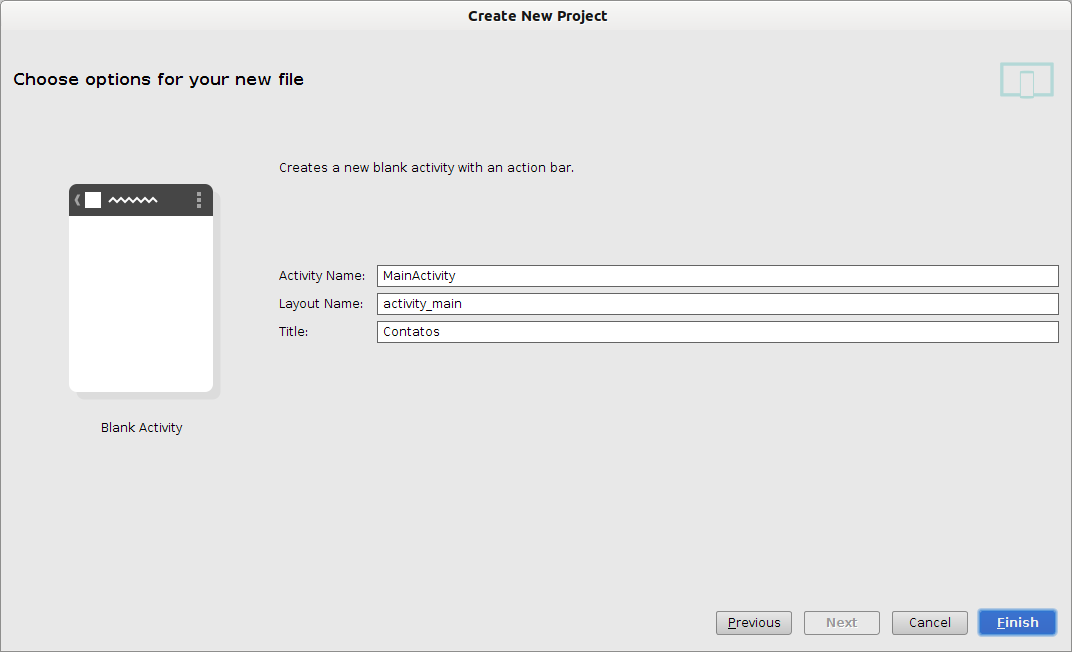
\includegraphics[scale=0.35]{img/exemplo-pratico/android-new-project-4.png}
    \caption{Novo projeto, tela 4}
    \label{fig:new-project-4}
\end{figure}

Este exemplo é bastante útil para aprendermos como funciona o Android.
Você só poderá criar algo se você souber utilizar bem as ferramentas.

\subsection{AndroidManifest.xml}

Este é o arquivo que define nossa aplicação, mapeia as
\texttt{Activity}'s, entre outras configurações. Ao finalizar a criação
do projeto, inicialmente este arquivo deverá conter o conteúdo descrito
no Código-fonte \ref{code:android-manifest-1}:

\begin{listing}[H]
  \inputminted[linenos=true,frame=bottomline,tabsize=3]{ xml }{ source/AndroidManifest-1.xml }
  \caption{Projeto inicial [AndroidManifest.xml]}
  \label{code:android-manifest-1}
\end{listing}

Devido a entrada do \gls{gradle} (ver
\href{http://www.gradleware.com/android/gradle-the-new-android-build-system/}{Gradle:
The New Android Build System}) a versão mínima e a versão alvo do SDK
foram movidas para o arquivo \texttt{build.gradle}. Outros detalhes em
\url{http://developer.android.com/sdk/installing/studio-build.html}.

\subsection{Activity \label{ssec:act}}

Não existe método \texttt{main} visível ao programador no Android. Ao
invés disso temos \texttt{Activity}'s. Para que o Android saiba qual ele
deve iniciar primeiro utilizamos um \texttt{intent-filter} como visto no
trecho de código acima da linha \circled{09} a \circled{12}. Para nossa
primeira \texttt{Activity} criaremos uma lista de contatos e um menu
para criação de um novo contato.

Para construir o \emph{layout} inicial de nossa aplicação precisamos
editar o arquivo \texttt{main.xml} localizado em \texttt{res/layout}.

\begin{listing}[H]
  \inputminted[linenos=true,frame=bottomline,tabsize=3]{ xml }{ source/main-1.xml }
  \caption{Layout principal [res/layout/main.xml]}
\end{listing}

Deste momento em diante tenha em mente que os arquivos \texttt{xml} aqui
descritos são apenas para você poder comparar e ver se não esqueceu de
nada. Todos os \emph{layout}'s devem ser criados usando a ferramenta
ADT. Você irá notar que ao abrir o \texttt{xml} uma janela de
\emph{layout} aparecerá. Para visualizar o \texttt{xml} ou o
\emph{layout} gráfico basta utilizar a aba inferior esquerda.

Por fim, temos o menu. Clique com o botão direito do \emph{mouse} em seu
projeto e \texttt{New} $\rightarrow$ \texttt{Other...} ou
\texttt{Ctrl + N}. Procure por \texttt{Android XML File}. Em
\texttt{Resource Type} escolha a opção \texttt{Menu}. Chame-o de
\texttt{main\_menu.xml}.

\begin{listing}[H]
  \inputminted[linenos=true,frame=bottomline,tabsize=3]{ xml }{ source/main_menu-1.xml }
  \caption{Menu principal [res/menu/main\b{ }menu.xml]}
\end{listing}

Pronto, já temos nosso layout. Compile o projeto e vamos a próxima
iteração.

\subsubsection{Convenção de nomes para ícones \label{sssec:nomeicones}}

Observe que o ícone utilizado no menu vem junto com o SDK do Android.
Você pode visualizar os ícones em
\texttt{SDK\_INSTALL/plataforms/android-8/data/res/drawable-hdpi}
(substitua \texttt{SDK\_INSTALL} pelo diretório de instalação do SDK do
Android, no nosso caso \texttt{usr/local/lib/android-sdk},
\ref{ssec:sdk}). Note que há \emph{namespaces} ou prefixos em cada um
dos ícones. O Android recomenda a seguinte convenção:

\ctable[caption = Convenção para nome dos ícones,
pos = H, center, botcap]{lll}
{% notes
}
{% rows
\FL
\parbox[b]{0.29\columnwidth}{\raggedright
\textbf{Tipo de Recurso}
} & \parbox[b]{0.26\columnwidth}{\raggedright
\textbf{Prefixo}
} & \parbox[b]{0.43\columnwidth}{\raggedright
\textbf{Exemplo}
}
\ML
\parbox[t]{0.29\columnwidth}{\raggedright
Ícones
} & \parbox[t]{0.26\columnwidth}{\raggedright
\texttt{ic\_}
} & \parbox[t]{0.43\columnwidth}{\raggedright
\texttt{ic\_adicionar.png}
}
\\\noalign{\medskip}
\parbox[t]{0.29\columnwidth}{\raggedright
Launcher icons
} & \parbox[t]{0.26\columnwidth}{\raggedright
\texttt{ic\_launcher\_}
} & \parbox[t]{0.43\columnwidth}{\raggedright
\texttt{ic\_launcher\_calendario.png}
}
\\\noalign{\medskip}
\parbox[t]{0.29\columnwidth}{\raggedright
Menu e Action Bar
} & \parbox[t]{0.26\columnwidth}{\raggedright
\texttt{ic\_menu\_}
} & \parbox[t]{0.43\columnwidth}{\raggedright
\texttt{ic\_menu\_ajuda.png}
}
\\\noalign{\medskip}
\parbox[t]{0.29\columnwidth}{\raggedright
Status bar icons
} & \parbox[t]{0.26\columnwidth}{\raggedright
\texttt{ic\_stat\_notify\_}
} & \parbox[t]{0.43\columnwidth}{\raggedright
\texttt{ic\_stat\_notify\_msg.png}
}
\\\noalign{\medskip}
\parbox[t]{0.29\columnwidth}{\raggedright
Tab icons
} & \parbox[t]{0.26\columnwidth}{\raggedright
\texttt{ic\_tab\_}
} & \parbox[t]{0.43\columnwidth}{\raggedright
\texttt{ic\_tab\_recente.png}
}
\\\noalign{\medskip}
\parbox[t]{0.29\columnwidth}{\raggedright
Dialog icons
} & \parbox[t]{0.26\columnwidth}{\raggedright
\texttt{ic\_dialog\_}
} & \parbox[t]{0.43\columnwidth}{\raggedright
\texttt{ic\_dialog\_info.png}
}
\LL
}

Note que você não é obrigado a utilizar os prefixos citados acima, isto
é apenas uma convenção. Veja mais detalhes em
\url{http://developer.android.com/guide/practices/ui_guidelines/icon_design.html}.

Abra o arquivo \texttt{MainActivity.java} e vá ao método
\texttt{onCreate}. Defina o \emph{layout} como sendo nosso
\texttt{main.xml}. Para isso adicione o \emph{layout} \textbf{main} ao
final do método:

\begin{listing}[H]
  \inputminted[linenos=true,frame=bottomline,tabsize=3]{ java }{ source/MainActivity-1.java }
  \caption{Definir layout [MainActivity.java]}
\end{listing}

\paragraph{Cuidado \label{par:r}}

no ambiente Android temos uma classe chamada \texttt{R}. Ela existe
tanto na biblioteca do Android como em cada projeto. Nesse caso faça o
\emph{import} da classe \texttt{contatos.app.R}. A classe
\texttt{android.R} é utilizada em outras situações, onde códigos
pré-prontos foram disponibilizados pela equipe do Android.

Agora precisamos sobrescrever os métodos \texttt{onCreateOptionsMenu} e
\texttt{onOptionsItemSelected}. Eles irão criar o menu a partir de nosso
\emph{layout} e notificar quando os itens do menu forem pressionados,
respectivamente. Vamos ao código:

\begin{listing}[H]
  \inputminted[linenos=true,frame=bottomline,tabsize=3]{ java }{ source/MainActivity-2.java }
  \caption{Criando o menu [MainActivity.java]}
\end{listing}

\subsection{Formulários}

Agora vamos criar nosso formulário para criação e edição de contatos.
Começaremos pelo \emph{layout}. Crie um arquivo \texttt{xml} em
\texttt{res/layout} chamado \texttt{salvar.xml}.

Existem alguns pontos importantes para este trecho de código. Começando
pelo \emph{layout} inicial, onde usaremos \texttt{TableLayout}. Esse
\emph{layout} é ideal para telas com estilo tabela.

Um detalhe importante para observarmos neste \emph{layout} é que ele
possui o atributo \texttt{stretchColumns} com valor \texttt{1}. Isso
quer dizer que a coluna \texttt{1} da tabela terá o maior tamanho
possível, respeitando o tamanho mínimo das outras células. Para
visualizar as mudanças você pode tentar usar outros valores como
\texttt{0} tornando a primeira coluna maior que as demais, ou ainda
\texttt{*} que fará com que todas as células tenham o mesmo tamanho.

\begin{listing}[H]
  \inputminted[linenos=true,frame=bottomline,tabsize=3]{ xml }{ source/salvar-1.xml }
  \caption{Formulário principal [res/layout/salvar.xml]}
\end{listing}

Crie uma nova \texttt{Activity} chamada \texttt{SalvarActivity} dentro
de \texttt{contatos.app.view}. Para irmos de uma \texttt{Activity} para
outra precisamos de um \texttt{Intent}. Um de seus construtores recebe
como parâmetros a instância da classe em que estamos, sendo que ela deve
implementar a interface \texttt{Context} e o nome da classe a qual deve
ser mostrada. Veja como implementar o método \texttt{irParaSalvar} da
classe \texttt{MainActivity}:

\begin{listing}[H]
  \inputminted[linenos=true,frame=bottomline,tabsize=3]{ java }{ source/MainActivity-3.java }
  \caption{Mudando de Activity [MainActivity.java]}
\end{listing}

Veremos agora como manipular \texttt{EditText}'s, que representam os
campos de entrada de dados. Abra o \texttt{SalvarActivity} e adicione o
método carregar e crie atributos para guardar os \texttt{EditText}'s:

\begin{listing}[H]
  \inputminted[linenos=true,frame=bottomline,tabsize=3]{ java }{ source/SalvarActivity-1.java }
  \caption{Utilizando EditText's [SalvarActivity.java]}
\end{listing}

Para que a \texttt{Activity} funcione precisamos mapeá-la no arquivo
\texttt{AndroidManifest.xml}. Adicione o conteúdo abaixo entre as
\emph{tags} \texttt{application}:

\begin{listing}[H]
  \inputminted[linenos=true,frame=bottomline,tabsize=3]{ xml }{ source/AndroidManifest-2.xml }
  \caption{Mapear SalvarActivity [AndroidManifest.xml]}
\end{listing}

Utilize sempre o ADT e apenas confira se o arquivo está da maneira
correta.

\subsection{Construindo o Model da aplicação \label{ssec:model}}

Precisamos de um \emph{helper} para fazer acesso ao banco de dados. O
Android provê suporte a bancos de dados
\href{http://sqlite.org/}{Sqlite} por padrão. Qualquer banco de dados
que você criar será acessível pelo nome por qualquer classe na sua
aplicação, mas não fora dela.

Crie uma classe chamada \texttt{ContatoHelper} em
\texttt{contatos.app.model} que extende de \texttt{SQLiteOpenHelper}.
Essa classe será capaz de ler e escrever no banco de dados graças aos
métodos \texttt{getReadableDatabase()} e \texttt{getWritableDatabase()},
respectivamente.

A princípio temos que criar um construtor passando como parâmetros o
nome do banco de dados e a versão da \gls{ddl} (\emph{Data Definition
Language}). Logo em seguida precisamos implementar os métodos
\texttt{onCreate}, no qual iremos criar as tabelas e \texttt{onUpdate},
caso tenhamos que alterar alguma tabela em versões futuras do
aplicativo.

\begin{listing}[H]
  \inputminted[linenos=true,frame=bottomline,tabsize=3]{ java }{ source/ContatoHelper-1.java }
  \caption{Helper da aplicação [ContatoHelper.java]}
\end{listing}

Para a iteração de criação de um novo contato, ainda em
\texttt{ContatoHelper} vamos adicionar um método \texttt{criar}. Faça:

\begin{listing}[H]
  \inputminted[linenos=true,frame=bottomline,tabsize=3]{ java }{ source/ContatoHelper-2.java }
  \caption{Criar novo contato [ContatoHelper.java]}
\end{listing}

Agora temos que fazer a chamada do método criar da classe
\texttt{ContatoHelper} em \texttt{SalvarActivity}. Para isso temos que
criar uma instância de \texttt{ContatoHelper}, adicionar o botão salvar
e adicionar um \emph{Listener} de \emph{click} (faça o \emph{import} da
classe \newline
\texttt{android.view.View.OnClickListener}). Vamos ao código:

\begin{listing}[H]
  \inputminted[linenos=true,frame=bottomline,tabsize=3]{ java }{ source/SalvarActivity-2.java }
  \caption{Fim da iteração criar contato [SalvarActivity.java]}
\end{listing}

Com essa implementação já é possível salvar contatos na base de dados.

\subsection{Mostrando os dados na View \label{ssec:listview}}

Após salvar os dados no banco, devemos ser capazes de obter tais
informações e colocá-las em forma de Lista. Para isso criaremos um novo
\emph{layout} que será responsável por representar uma linha de nossa
Lista. Essa linha deve ser semelhante a figura abaixo:

\begin{figure}[h]
    \centering
    \includegraphics[scale=0.6]{img/layout-linha.png}
    \caption{Layout linha da Lista}
\end{figure}

Para isso crie um arquivo chamado \texttt{linha.xml} em
\texttt{res/layout} com o seguinte conteúdo.

\begin{listing}[H]
  \inputminted[linenos=true,frame=bottomline,tabsize=3]{ xml }{ source/linha-1.xml }
  \caption{Layout para cada linha da lista [res/layout/linha.xml]}
\end{listing}

Note a possibilidade de aninhar o \texttt{LinearLayout}. Fazendo isso é
possível criar o \emph{layout} desejado fazendo com que alguns elementos
sejam inseridos na horizontal, outros na vertical.

Outro ponto interessante é o uso de negrito no \texttt{TextView}
correspondente ao nome, na linha \circled{14}, e o uso de reticências
caso o nome seja maior que a tela usando
\texttt{android:ellipsize="end"} na linha \circled{15}.

Agora vamos até \texttt{ContatoHelper} e adicionar o método
\texttt{listar}. E também adicionaremos métodos para facilitar a
obtenção dos valores de cada atributo.

\begin{listing}[H]
  \inputminted[linenos=true,frame=bottomline,tabsize=3]{ java }{ source/ContatoHelper-3.java }
  \caption{Listar contatos existentes [ContatoHelper.java]}
\end{listing}

Os elementos de um \texttt{Cursor} são numerados iniciando de 0 (zero).
Neste caso o 0 é a coluna \texttt{\_id}. Observe que ela não será usada
pelo programador e sim pelo Android. Isto será visto com mais detalhes
em \ref{ssec:edit} Editando dados existentes.

Para popular cada linha de nossa Lista vamos criar uma classe interna
(\emph{inner class}) em \texttt{MainActivity}. Assim podemos fazer
\emph{cache} dos objetos aumentando a performance. Use o sufixo
\texttt{Holder} para esse tipo de classe.

\begin{listing}[H]
  \inputminted[linenos=true,frame=bottomline,tabsize=3]{ java }{ source/MainActivity-4.java }
  \caption{Classe Holder [MainActivity.java]}
\end{listing}

Levando em conta que estamos usando a interface \texttt{Cursor} em nosso
\texttt{Helper} temos que criar uma classe que extenda de
\texttt{CursorAdapter} que será responsável por definir o \emph{layout}
de cada linha da Lista. Crie uma classe interna chamada
\texttt{ContatoAdapter}. Iremos sobrescrever dois métodos,
\texttt{newView()} e \texttt{bindView()}, que são responsáveis por
inflar (\emph{inflate}) uma nova linha e reciclar uma linha existente,
respectivamente.

\begin{listing}[H]
  \inputminted[linenos=true,frame=bottomline,tabsize=3]{ java }{ source/MainActivity-5.java }
  \caption{Classe Adapter [MainActivity.java]}
\end{listing}

Com a introdução do \texttt{Helper} teremos que criar uma instância da
classe \texttt{Cursor} para popular nossa \texttt{ListView}. Vamos ao
código-fonte:

\begin{listing}[H]
  \inputminted[linenos=true,frame=bottomline,tabsize=3]{ java }{ source/MainActivity-6.java }
  \caption{Popular ListView [MainActivity.java]}
\end{listing}

Nunca esquecendo de fechar o \texttt{helper} ao sair, pois assim
garantimos que a conexão com o banco será fechada.

\subsection{Editando dados existentes \label{ssec:edit}}

Para a edição de informações usaremos o mesmo \texttt{Activity} que
usamos para criar um contato, ou seja, \texttt{SalvarActivity}. Mas para
isso precisamos passar um parâmetro para o \texttt{Activity}. Usaremos
então um método do \texttt{Intent} que é responsável por isso,
\texttt{putExtra(chave, valor)}.

Para uma passagem de parâmetros segura devemos usar um \emph{namespace}
para que não colida com nenhum nome já utilizado pelo Android. Assim,
vamos criar uma variável estática do tipo \texttt{String}. Isso
acontecerá quando o usuário pressionar a linha que ele deseja editar.
Podemos fazer isso utilizando a interface \texttt{OnItemClickListener}.

Vamos incrementar também o método \texttt{irParaSalvar} passando o
parâmetro caso haja um. Vamos ao código:

\begin{listing}[H]
  \inputminted[linenos=true,frame=bottomline,tabsize=3]{ java }{ source/MainActivity-7.java }
  \caption{Passagem de parâmetros [MainActivity.java]}
\end{listing}

Agora é hora de tratar nosso parâmetro no \texttt{SalvarActivity}. Caso
haja um parâmetro precisamos obter os dados existentes no banco de dados
para então editá-lo. Neste caso precisaremos de mais dois métodos em
\texttt{ContatoHelper}, que são \texttt{ler} e \texttt{atualizar}.

\begin{listing}[H]
  \inputminted[linenos=true,frame=bottomline,tabsize=3]{ java }{ source/ContatoHelper-4.java }
  \caption{Ler e atualizar dados existentes [ContatoHelper.java]}
\end{listing}

O próximo passo é tratar no \texttt{SalvarActivity} caso o parâmetro
tenha sido enviado ou não. Caso positivo devemos carregar os dados
existentes no banco de dados e depois atualizá-los.

\begin{listing}[H]
  \inputminted[linenos=true,frame=bottomline,tabsize=3]{ java }{ source/SalvarActivity-3.java }
  \caption{Usando Activity para criar ou atualizar [SalvarActivity.java]}
\end{listing}

Com isso encerramos um \textbf{CRUD} básico, mas completo. A seguir
temos implementações mais específicas que irão tornar nossa aplicação
mais profissional.
